\documentclass{beamer}
\usepackage{lmodern}
\usepackage[utf8]{inputenc}

\usepackage{enumerate}
\usepackage{multimedia}

\usetheme{polimix}
 
\title[Adaptive Policy Search]{Adaptive Policy Search}
\subtitle{First Annual Report}

\author[M. Papini]{Matteo Papini}
\supervisor{Supervisor}{Marcello Restelli}
\date[19/9/2018]{19 Settembre 2018}

\begin{document}

%%%%%%%%%%%%%%%%%%%%%%%%%%%%%%%%%%%%%%%%%%%%%%%%%%%%%%%%%%%%%%%%%%%%%%%%%%%%%%%%%%%%%%%%%%%%%%%%%%%%%%%%%%%%%%%%%%%%

\begin{frame}
\titlepage
\end{frame}

\addtocounter{framenumber}{-1}

%%%%%%%%%%%%%%%%%%%%%%%%%%%%%%%%%%%%%%%%%%%%%%%%%%%%%%%%%%%%%%%%%%%%%%%%%%%%%%%%%%%%%%%%%%%%%%%%%%%%%%%%%%%%%%%%%%%%

%\begin{frame}
%\frametitle{Sommario}
%\tableofcontents
%\end{frame}

%%%%%%%%%%%%%%%%%%%%%%%%%%%%%%%%%%%%%%%%%%%%%%%%%%%%%%%%%%%%%%%%%%%%%%%%%%%%%%%%%%%%%%%%%%%%%%%%%%%%%%%%%%%%%%%%%%%
\section{Overview}

\begin{frame}
\frametitle{Motivation}
Design \textbf{efficient} and \textbf{reliable} controllers for real-world problems (robotics, industrial processes...) where accurate models are not available

\vfill

\textbf{Reinforcement Learning (RL)~\cite{sutton1998reinforcement}} is a powerful technique for model-free control and achieved great results in \textit{games}. To tackle real problems, we need RL methods that are:

\vfill

\begin{columns}
	\begin{column}{.6\textwidth}
		\begin{itemize}
			\item \textbf{Continuous}
			\item \textbf{Safe}
			\item \textbf{Sample-efficient}
		\end{itemize}
	\end{column}
	\begin{column}{.4\textwidth}
		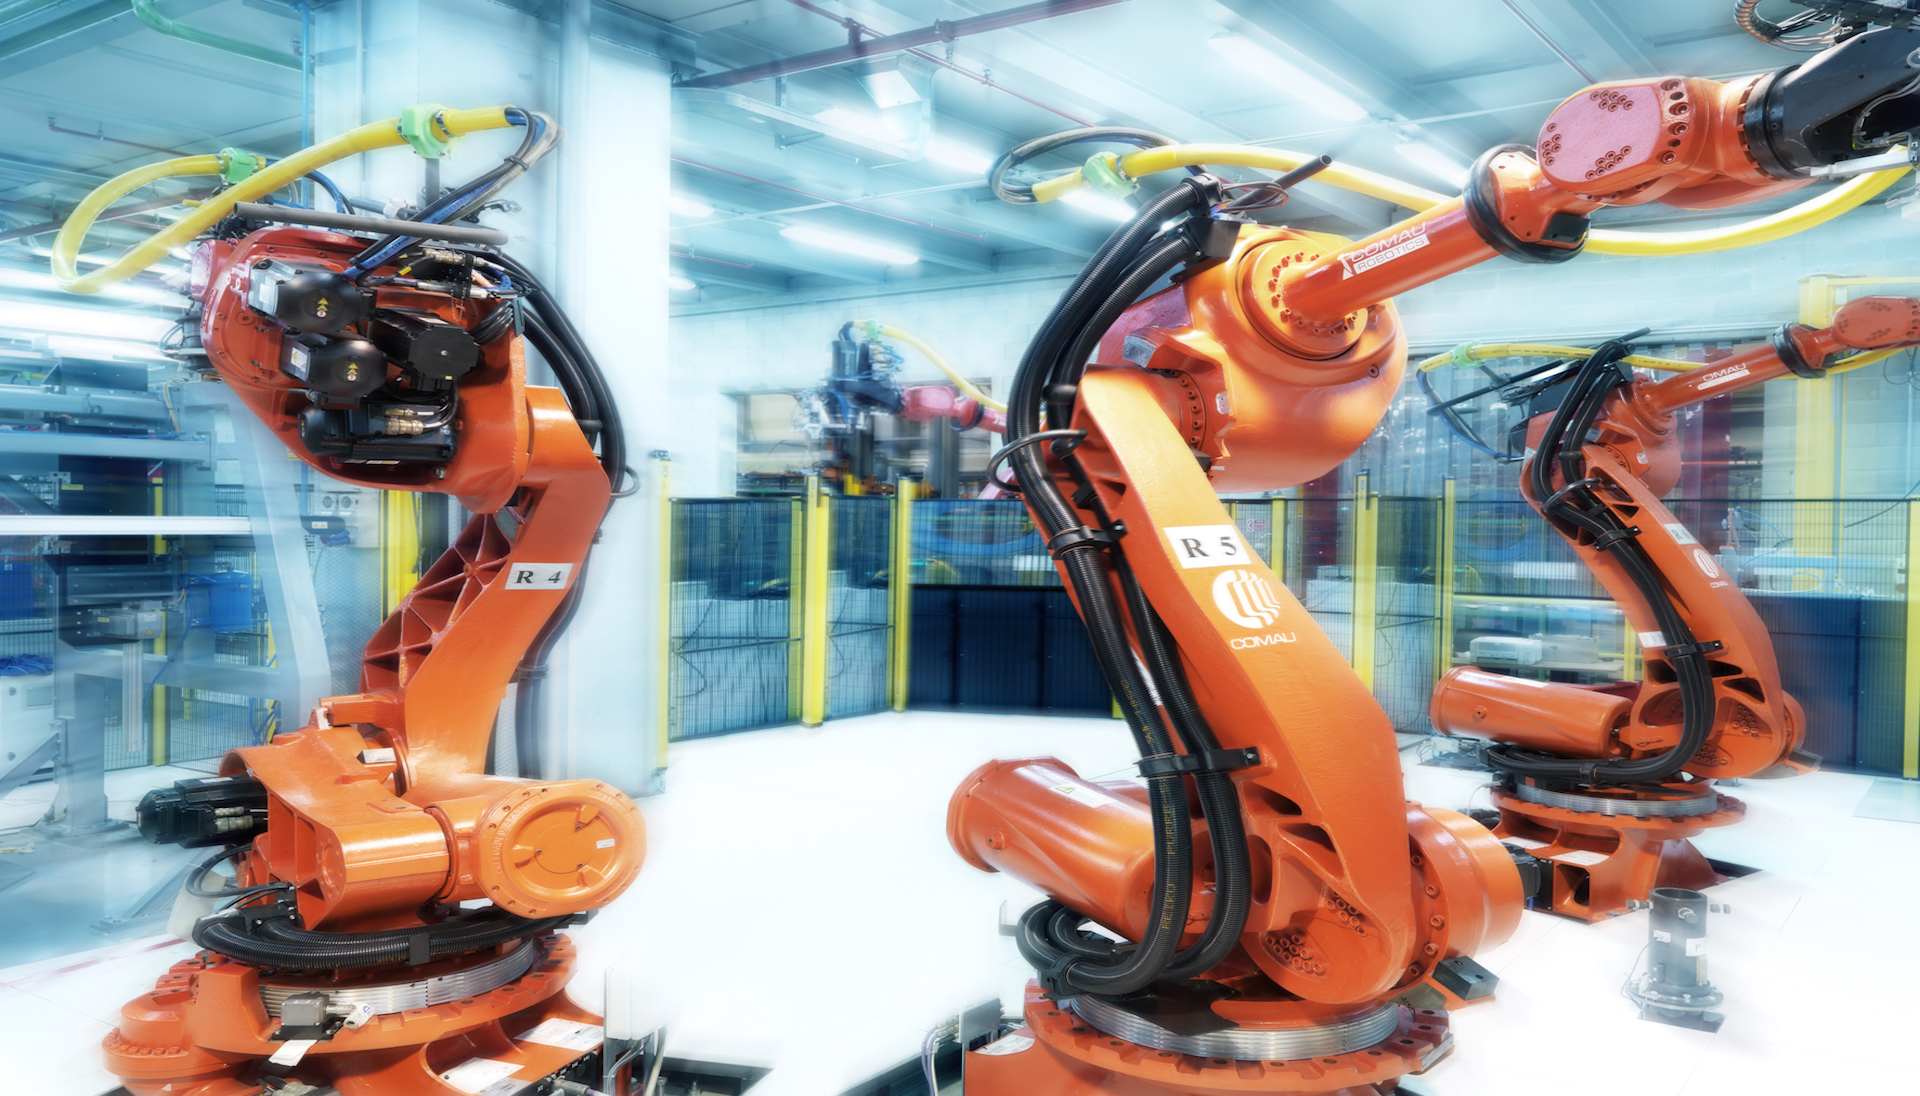
\includegraphics[width=\textwidth]{pics/robots.jpg}
	\end{column}
\end{columns}


\end{frame}


\begin{frame}
\frametitle{Policy Search \cite{deisenroth2013survey}}

Search for the policy $\pi \in \Pi$ that maximizes the expected sum of rewards ${J(\pi) = \mathop{E_{\pi}}\left[\sum_{t=0}^{T}\gamma^tr_t\right]}$

\vfill

\begin{center}
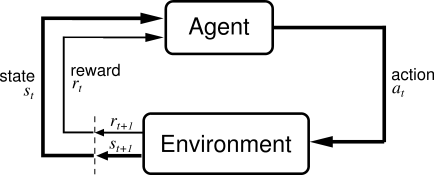
\includegraphics[width=.5\textwidth]{pics/rl.png}
\end{center}

\vfill

Can manage \textbf{continuous} states and action spaces

\vfill

\textbf{Policy Gradient (PG)}~\cite{sutton2000policy}:
\begin{itemize}
	\item Restrict the search to parametric policies $\pi_{\theta}$ where $\theta \in \Theta$
	\item Search via gradient ascent on $J(\theta)$
\end{itemize}

\end{frame}


\begin{frame}
\frametitle{Adaptive Policy Search}

\textbf{Adaptation} is needed to trade-off competing aspects of learning on real systems:

\vspace{5pt}

\begin{itemize}
	\item Safety and efficiency
	\item Exploration and safety
	\item Exploration and efficiency
\end{itemize}

\vfill

and to autonomously react to:

\vspace{5pt}

\begin{itemize}
	\item Changes in the external conditions
	\item Changes in the objectives
\end{itemize}

\end{frame}

%%%%%%%%%%%%%%%%%%%%%%%%%%%%%%%%%%%%%%%%%%%%%%%%%%%%%%%%%%%%%%%%%%%%%%%%%%%%%%%%%%%%%%%%%%%%%%%%%%%%%%%%%%%%%%%%%%%
\section{Safety}


\begin{frame}
\frametitle{Safe Policy Gradient}

"Safety" is used with many meanings in the literature \cite{garcia2015comprehensive}. We focus on \textbf{performance guarantees}~\cite{kakade2002approximately, thomas2015high}, either with a danger-avoidance or an economic meaning:

\begin{align*}
	J(\theta') - J(\theta) \geq C \quad\text{ in high probability}
\end{align*}

In \textbf{policy gradient} safety can be ensured with an \textbf{adaptive step size}~\cite{pirotta2013adaptive}:

\begin{align*}
	\theta' = \theta + \textcolor{red}{\mathbf{\alpha}}\widehat{\nabla}_{\theta}J(\theta)
\end{align*}

A small $\alpha$ is safe, but slows down convergence. The adaptive algorithm can find the best value for each iteration. 

\end{frame}


\begin{frame}
\frametitle{Adaptive Batch Size for Safe Policy Gradient~\cite{papini2017adaptive}}
Idea: also adapt the \textbf{batch size} used to estimate the gradient

\begin{align*}
	\widehat{\nabla}_{\theta}^NJ(\theta) = \frac{1}{\textcolor{red}{\mathbf{N}}}\sum_{i=0}^{N}\underbrace{\textcolor{lightgray}{\left[\sum_{t=0}^T\left(\sum_{h=0}^t\nabla_{\theta}\log\pi_{\theta}(a_h^i\mid s_h^i)\right) \gamma^tr_t\right]}}_{\text{gradient information from $i$-th episode of experience}}
\end{align*}

A large batch size is safe, but is inefficient.

\vfill

Contributions:
\begin{itemize}
	\item We show that \textbf{coordinate ascent} yields better guarantees than gradient ascent
	\item We show an interesting duality between step size and batch size
	\item We provide an adaptive batch size to trade-off safety and efficiency
\end{itemize}

\end{frame}


\begin{frame}
\frametitle{Safely Exploring Policy Gradient}
Existing guarantees are on \textbf{Gaussian policies} with fixed variance:
\begin{align*}
	\pi_{\theta}(a \vert s) = \mathcal{N}(\mu_{\theta}(s), \textcolor{red}{\mathbf{\sigma}})
\end{align*}

Policy variance controls \textbf{exploration}: random behavior used to collect novel information $\implies$ potentially \textbf{unsafe}

\vfill

\textbf{Idea}: also learn the variance via adaptive PG to achieve \textbf{safe exploration}~\cite{amodei2016concrete}.

\vfill

Contributions:
\begin{itemize}
	\item We generalize safety requirements to model \textit{more practical} scenarios, such as the \textbf{fine-tuning} of handcrafted controllers
	\item We introduce a surrogate objective that encodes the \textbf{long-term advantages} of exploration
	\item We extend safety guarantees to the learned-variance case
\end{itemize}
\end{frame}


\begin{frame}
\frametitle{Safe Policy Gradient: Frontiers}
In more recent work:
\begin{itemize}
	\item We provide \textbf{general safety guarantees} that do \textit{not} assume a specific class of policies. The general policy requirements are:
	
	\begin{align*}
		&\sup_{s}\mathop{E}_{a\sim\pi_{\theta}}\left[\left|\nabla_{\theta}\log\pi_{\theta}(a\vert s)\right|\right] < \infty \\
		&\sup_{s}\mathop{E}_{a\sim\pi_{\theta}}\left[\left|\nabla_{\theta}\log\pi_{\theta}(a\vert s)\nabla_{\theta}\log\pi_{\theta}(a\vert s)^T\right|\right] < \infty \\
		&\sup_{s}\mathop{E}_{a\sim\pi_{\theta}}\left[\left|\mathop{Hess}\left(\log\pi_{\theta}(a\vert s)\right)\right|\right] < \infty \\
	\end{align*}
	
	\item We further study the \textbf{convergence properties} of policy gradient methods
\end{itemize}

\end{frame}

%%%%%%%%%%%%%%%%%%%%%%%%%%%%%%%%%%%%%%%%%%%%%%%%%%%%%%%%%%%%%%%%%%%%%%%%%%%%%%%%%%%%%%%%%%%%%%%%%%%%%%%%%%%%%%%%%%%
\section{Sample Efficiency}


\begin{frame}
\frametitle{Stochastic Variance-Reduced Policy Gradient~\cite{papini2018stochastic}}
Sample inefficiency is the main obstacle to real-world applications of policy search~\cite{recht2018tour}, and is made even worse by safety requirements

\vfill

Recent optimization techniques, such as \textbf{SVRG}~\cite{johnson2013accelerating}, combine accurate and inaccurate gradient estimations to achieve a better \textbf{effective convergence rate}

\vfill

\begin{columns}
	\begin{column}{0.59\textwidth}
		Idea: apply SVRG to policy gradient
		\scriptsize
		\begin{align*}
			\blacktriangledown_{\theta}J(\theta) = \widehat{\nabla}_{\theta}^NJ(\widetilde{\theta}) + \widehat{\nabla}_{\theta}^BJ(\theta) - w(\theta,\widetilde{\theta})\widehat{\nabla}_{\theta}^BJ(\theta)
		\end{align*}
	\end{column}
	\begin{column}{0.29\textwidth}
		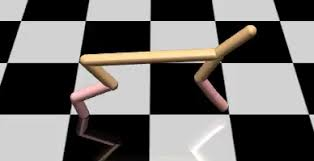
\includegraphics[width=\textwidth]{pics/cheetah.jpeg}
	\end{column}
\end{columns}

\vfill

Contributions:
\begin{itemize}
	\item We analyze the potential and challenges of SVRG in RL
	\item We propose an SVRG-based policy gradient algorithm
	\item We prove a theoretical \textbf{rate of convergence}
	\item We empirically show advantages over naive optimization
\end{itemize}

\end{frame}


\begin{frame}
\frametitle{Policy Optimization via Importance Sampling}
Reusing the same data for multiple updates (\textbf{off-policy learning}) can improve \textbf{sample efficiency}

\vfill

Unfortunately, updates degrade as the target policy $\pi_{\theta}$ goes further away from the one used to collect data $\pi_{\tilde{\theta}}$ (\textbf{covariate shift})

\vfill

Idea: penalize \textbf{divergence} in the learning objective
\begin{align*}
	\mathcal{L}(\theta) = w(\widetilde{\theta},\theta)\nabla_{\theta}^NJ(\theta) - \frac{\lambda}{N}d(\pi_{\theta}, \pi_{\tilde{\theta}})
\end{align*}

Contributions:
\begin{itemize}
	\item We propose a surrogate objective with strong theoretical motivations
	\item We consider both \textbf{control-based} and \textbf{parameter-based} optimization
	\item We improve over state-of-the-art (TRPO~\cite{schulman2015trust}) in several benchmark tasks
\end{itemize}

\end{frame}

%%%%%%%%%%%%%%%%%%%%%%%%%%%%%%%%%%%%%%%%%%%%%%%%%%%%%%%%%%%%%%%%%%%%%%%%%%%%%%%%%%%%%%%%%%%%%%%%%%%%%%%%%%%%%%%%%%%
\section{Conclusion}


\begin{frame}
\frametitle{Future Work}

Short term (one year):
\begin{itemize}
	\item Study the problem of \textbf{exploration} in more depth to better capture the costs and advantages of exploratory behavior
\end{itemize}

\vfill

Long term (two years):
\begin{itemize}
	\item \textbf{Unify} the proposed methods to achieve efficient safe exploration
	\item Tackle more challenging and \textbf{realistic} problems
\end{itemize}

\vfill

\begin{columns}
	\begin{column}{0.35\textwidth}
		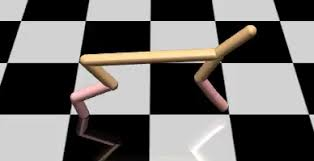
\includegraphics[height=50pt]{pics/cheetah.jpeg}
	\end{column}
%	\begin{column}{0.49\textwidth}
%		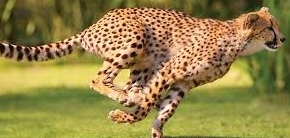
\includegraphics[height=50pt]{pics/real_cheetah.jpg}
%	\end{column}
	\begin{column}{0.1\textwidth}
		\centering
		\LARGE$\to$
	\end{column}
	\begin{column}{0.35\textwidth}
	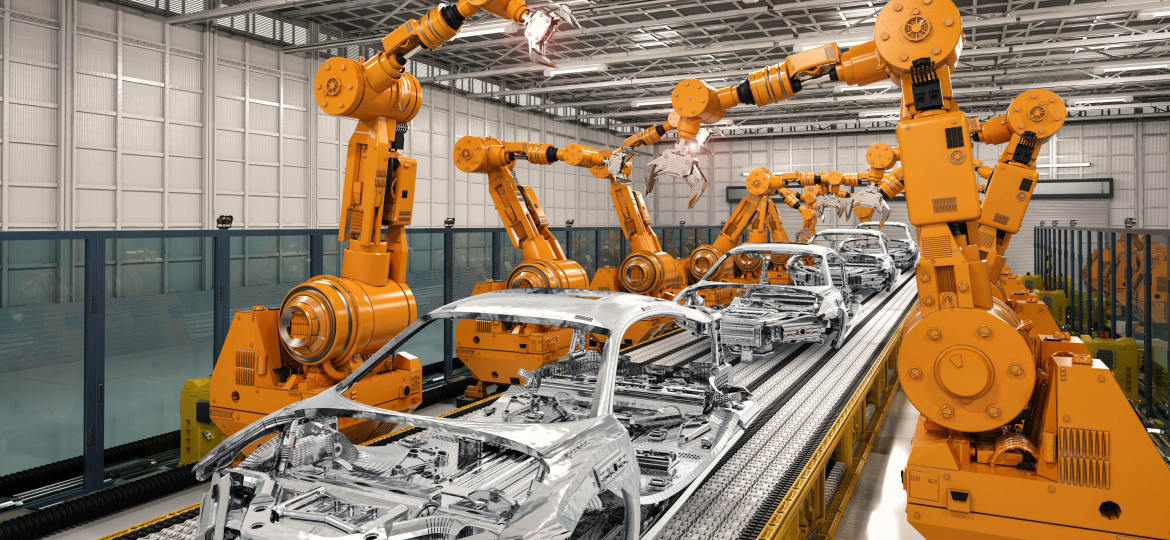
\includegraphics[height=50pt]{pics/factory.jpg}
	\end{column}
\end{columns}

\end{frame}


\begin{frame}
\frametitle{Attended Courses and Schools}


\end{frame}


\begin{frame}
\frametitle{Publications and Submissions}


\end{frame}


\begin{frame}
\frametitle{Other Activities}


\end{frame}

%%%%%%%%%%%%%%%%%%%%%%%%%%%%%%%%%%%%%%%%%%%%%%%%%%%%%%%%%%%%%%%%%%%%%%%%%%%%%%%%%%%%%%%%%%%%%%%%%%%%%%%%%%%%%%%%%%%

\begin{frame}[allowframebreaks]
\frametitle{Bibliography}
\bibliographystyle{brev}
\bibliography{slides}

\end{frame}

%%%%%%%%%%%%%%%%%%%%%%%%%%%%%%%%%%%%%%%%%%%%%%%%%%%%%%%%%%%%%%%%%%%%%%%%%%%%%%%%%%%%%%%%%%%%%%%%%%%%%%%%%%%%%%%%%%%


\end{document} 
